\begin{figure}[!ht]
\centering
\resizebox{0.75\textwidth}{!}{%
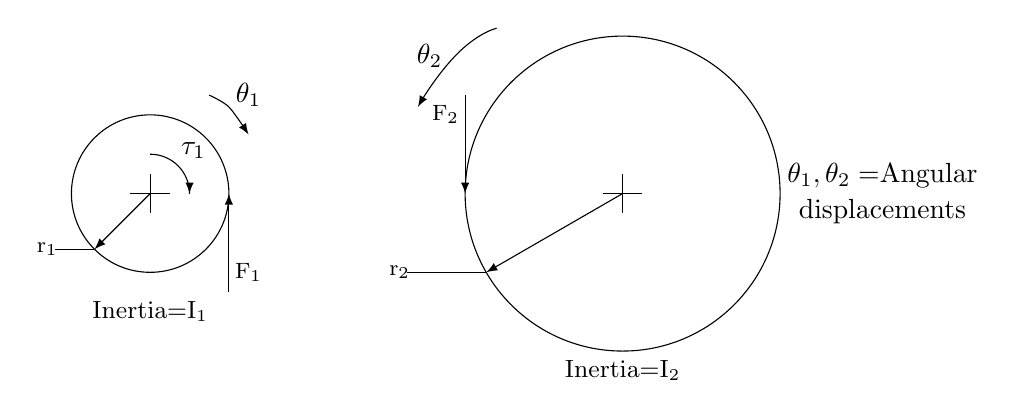
\begin{tikzpicture}
    \draw[black] (-2,0) circle (1);
    \node at (-2,-1.5){\small Inertia=I$_1$};
    \draw[black] (4,0) circle (2);
    \node at (4, -2.25){\small Inertia=I$_2$};
    \draw[black] (-2,0.25) to (-2,-0.25);
    \draw[black] (-1.75,0) to (-2.25,0);
    \draw[black] (4,0.25) to (4,-0.25);
    \draw[black] (3.75,0) to (4.25,0);
    \draw[black, latex-] (-1,0) to (-1,-1.25);
    \node at (-0.75,-1){\footnotesize F$_1$};
    \draw[black, latex-] (2,0) to (2,1.25);
    \node at (1.75,+1){\footnotesize F$_2$};
    \draw[black, -latex] (4,0) to ++(-{sqrt(3)}, -1);
    \draw[black] ({4-sqrt(3)},-1) to ++(-1,0);
    \node[black] at ({2.9-sqrt(3)},-1){\footnotesize r$_2$};
    \draw[black, -latex] (-2,0) to ++(-{sqrt(0.5)},-{sqrt(0.5)});
    \draw[black] ({-2-sqrt(0.5)}, -{sqrt(0.5)}) to ++(-0.5,0);
    \node[black] at ({-2.6-sqrt(0.5)},{-sqrt(0.5)}){\footnotesize r$_1$};
    \draw[black] (-2, 0.5) arc[start angle=90, end angle=0, radius=0.5];
    \node at (-1.45,0.55){$\tau_1$};
    \draw[black, latex-] (-1.5,0) to ++(0,0.001);
    \node at (7.3,0.23) {$\theta_1,\theta_2=$Angular};
    \node at (7.3,-0.23) {displacements};
    \draw[black, -latex] plot[smooth] coordinates {(-1.25,1.25) (-1.00,1.1) (-
    0.75,0.75)};
    \node at (-0.75,1.25) {$\theta_1$};
    \draw[black, -latex] plot[smooth, tension=1] coordinates {(2.4,2.1) (1.9,1.775) (1.4,1.1)};
    \node at (1.55,1.75){$\theta_2$};
\end{tikzpicture}
}%

\label{fig:my_label}
\end{figure}